\documentclass[12pt]{extreport}
\usepackage[T2A]{fontenc}
\usepackage[utf8]{inputenc}        % Кодировка входного документа;
                                    % при необходимости, вместо cp1251
                                    % можно указать cp866 (Alt-кодировка
                                    % DOS) или koi8-r.

\usepackage[english,russian]{babel} % Включение русификации, русских и
                                    % английских стилей и переносов
%%\usepackage{a4}
%%\usepackage{moreverb}
\usepackage{amsmath,amsfonts,amsthm,amssymb,amsbsy,amstext,amscd,amsxtra,multicol,mathtools}
\usepackage{indentfirst}
\usepackage{verbatim}
\usepackage{tikz} %Рисование автоматов
\usetikzlibrary{automata,positioning}
\usepackage{multicol} %Несколько колонок
\usepackage{graphicx}
\usepackage[colorlinks,urlcolor=blue]{hyperref}
\usepackage[stable]{footmisc}

\usepackage[linesnumbered]{algorithm2e}   

%% \voffset-5mm
%% \def\baselinestretch{1.44}
\renewcommand{\theequation}{\arabic{equation}}
\def\hm#1{#1\nobreak\discretionary{}{\hbox{$#1$}}{}}
\newtheorem{Lemma}{Лемма}
\theoremstyle{definiton}
\newtheorem{Remark}{Замечание}
%%\newtheorem{Def}{Определение}
\newtheorem{Claim}{Утверждение}
\newtheorem{Cor}{Следствие}
\newtheorem{Theorem}{Теорема}
\theoremstyle{definition}
\newtheorem{Example}{Пример}
\newtheorem*{known}{Теорема}
\def\proofname{Доказательство}
\theoremstyle{definition}
\newtheorem{Def}{Определение}

%% \newenvironment{Example} % имя окружения
%% {\par\noindent{\bf Пример.}} % команды для \begin
%% {\hfill$\scriptstyle\qed$} % команды для \end






%\date{22 июня 2011 г.}
\let\leq\leqslant
\let\geq\geqslant
\def\MT{\mathrm{MT}}
%Обозначения ``ажуром''
\def\BB{\mathbb B}
\def\CC{\mathbb C}
\def\RR{\mathbb R}
\def\SS{\mathbb S}
\def\ZZ{\mathbb Z}
\def\NN{\mathbb N}
\def\FF{\mathbb F}
%греческие буквы
\let\epsilon\varepsilon
\let\es\varnothing
\let\eps\varepsilon
\let\al\alpha
\let\sg\sigma
\let\ga\gamma
\let\ph\varphi
\let\om\omega
\let\ld\lambda
\let\Ld\Lambda
\let\vk\varkappa
\let\Om\Omega
\def\abstractname{}

\def\R{{\cal R}}
\def\A{{\cal A}}
\def\B{{\cal B}}
\def\C{{\cal C}}
\def\D{{\cal D}}

%классы сложности
\def\REG{{\mathsf{REG}}}
\def\CFL{{\mathsf{CFL}}}


%%%%%%%%%%%%%%%%%%%%%%%%%%%%%%% Problems macros  %%%%%%%%%%%%%%%%%%%%%%%%%%%%%%%


%%%%%%%%%%%%%%%%%%%%%%%% Enumerations %%%%%%%%%%%%%%%%%%%%%%%%

\newcommand{\Rnum}[1]{\expandafter{\romannumeral #1\relax}}
\newcommand{\RNum}[1]{\uppercase\expandafter{\romannumeral #1\relax}}

%%%%%%%%%%%%%%%%%%%%% EOF Enumerations %%%%%%%%%%%%%%%%%%%%%

\usepackage{xparse}
\usepackage{ifthen}
\usepackage{bm} %%% bf in math mode
\usepackage{color}
%\usepackage[usenames,dvipsnames]{xcolor}

\definecolor{Gray555}{HTML}{555555}
\definecolor{Gray444}{HTML}{444444}
\definecolor{Gray333}{HTML}{333333}


\newcounter{problem}
\newcounter{uproblem}
\newcounter{subproblem}
\newcounter{prvar}

\def\beforPRskip{
	\bigskip
	%\vspace*{2ex}
}

\def\PRSUBskip{
	\medskip
}


\def\pr{\beforPRskip\noindent\stepcounter{problem}{\bf \theproblem .\;}\setcounter{subproblem}{0}}
\def\pru{\beforPRskip\noindent\stepcounter{problem}{\bf $\mathbf{\theproblem}^\circ$\!\!.\;}\setcounter{subproblem}{0}}
\def\prstar{\beforPRskip\noindent\stepcounter{problem}{\bf $\mathbf{\theproblem}^*$\negthickspace.}\setcounter{subproblem}{0}\;}
\def\prpfrom[#1]{\beforPRskip\noindent\stepcounter{problem}{\bf Задача \theproblem~(№#1 из задания).  }\setcounter{subproblem}{0} }
\def\prp{\beforPRskip\noindent\stepcounter{problem}{\bf Задача \theproblem .  }\setcounter{subproblem}{0} }

\def\prpvar{\beforPRskip\noindent\stepcounter{problem}\setcounter{prvar}{1}{\bf Задача \theproblem \;$\langle${\rm\Rnum{\theprvar}}$\rangle$.}\setcounter{subproblem}{0}\;}
\def\prpv{\beforPRskip\noindent\stepcounter{prvar}{\bf Задача \theproblem \,$\bm\langle$\bracketspace{{\rm\Rnum{\theprvar}}}$\bm\rangle$.  }\setcounter{subproblem}{0} }
\def\prv{\beforPRskip\noindent\stepcounter{prvar}{\bf \theproblem\,$\bm\langle$\bracketspace{{\rm\Rnum{\theprvar}}}$\bm\rangle$}.\setcounter{subproblem}{0} }

\def\prpstar{\beforPRskip\noindent\stepcounter{problem}{\bf Задача $\bf\theproblem^*$\negthickspace.  }\setcounter{subproblem}{0} }
\def\prdag{\beforPRskip\noindent\stepcounter{problem}{\bf Задача $\theproblem^{^\dagger}$\negthickspace\,.  }\setcounter{subproblem}{0} }
\def\upr{\beforPRskip\noindent\stepcounter{uproblem}{\bf Упражнение \theuproblem.}\setcounter{subproblem}{0}\;}
%\def\prp{\vspace{5pt}\stepcounter{problem}{\bf Задача \theproblem .  } }
%\def\prs{\vspace{5pt}\stepcounter{problem}{\bf \theproblem .*   }
\def\prsub{\PRSUBskip\noindent\stepcounter{subproblem}{\sf \thesubproblem.}\;}
\def\prsubr{\PRSUBskip\noindent\stepcounter{subproblem}{\bf \asbuk{subproblem})}\;}
\def\prsubstar{\PRSUBskip\noindent\stepcounter{subproblem}{\rm $\thesubproblem^*$\negthickspace.}\;}
\def\prsubrstar{\PRSUBskip\noindent\stepcounter{subproblem}{$\text{\bf \asbuk{subproblem}}^*\mathbf{)}$}\;}

\newcommand{\bracketspace}[1]{\phantom{(}\!\!{#1}\!\!\phantom{)}}

\DeclareDocumentCommand{\Prpvar}{ O{null} O{} }{
	\beforPRskip\noindent\stepcounter{problem}\setcounter{prvar}{1}{\bf Задача \theproblem
% 	\ifthenelse{\equal{#1}{null}}{  }{ {\sf $\bm\langle$\bracketspace{#1}$\bm\rangle$}}
%	~\!\!(\bracketspace{{\rm\Rnum{\theprvar}}}).  }\setcounter{subproblem}{0}
%	\;(\bracketspace{{\rm\Rnum{\theprvar}}})}\setcounter{subproblem}{0}
%
	\,{\sf $\bm\langle$\bracketspace{{\rm\Rnum{\theprvar}}}$\bm\rangle$}
	~\!\!\! \ifthenelse{\equal{#1}{null}}{\!}{{\sf(\bracketspace{#1})}}}.

}
%\DeclareDocumentCommand{\Prpvar}{ O{level} O{meta} m }{\prpvar}


\DeclareDocumentCommand{\Prp}{ O{null} O{null} }{\setcounter{subproblem}{0}
	\beforPRskip\noindent\stepcounter{problem}\setcounter{prvar}{0}{\bf Задача \theproblem
	~\!\!\! \ifthenelse{\equal{#1}{null}}{\!}{{\sf(\bracketspace{#1})}}
	 \ifthenelse{\equal{#2}{null}}{\!\!}{{\sf [\color{Gray444}\,\bracketspace{{\fontfamily{afd}\selectfont#2}}\,]}}}.}

\DeclareDocumentCommand{\Pr}{ O{null} O{null} }{\setcounter{subproblem}{0}
	\beforPRskip\noindent\stepcounter{problem}\setcounter{prvar}{0}{\bf\theproblem
	~\!\! \ifthenelse{\equal{#1}{null}}{\!\!}{{\sf(\bracketspace{#1})}}
	 \ifthenelse{\equal{#2}{null}}{\!\!}{{\sf [\color{Gray444}\,\bracketspace{{\fontfamily{afd}\selectfont#2}}\,]}}}.}
	
	\DeclareDocumentCommand{\Prstar}{ O{null} O{null} }{\setcounter{subproblem}{0}
			\medskip\noindent\stepcounter{problem}\setcounter{prvar}{0}{\bf$\mathbf{\theproblem^*}$
			~\!\!\! \ifthenelse{\equal{#1}{null}}{\!}{{\sf(\bracketspace{#1})}}
			 \ifthenelse{\equal{#2}{null}}{\!\!}{{\sf [\color{Gray444}\,\bracketspace{{\fontfamily{afd}\selectfont#2}}\,]}}}.}
	

%\DeclareDocumentCommand{\Prp}{ O{level} O{meta} }

\DeclareDocumentCommand{\Prps}{ O{null} O{null} }{\setcounter{subproblem}{0}
	\beforPRskip\noindent\stepcounter{problem}\setcounter{prvar}{0}{\bf Задача $\bm\theproblem^* $
	~\!\!\! \ifthenelse{\equal{#1}{null}}{\!}{{\sf(\bracketspace{#1})}}
	 \ifthenelse{\equal{#2}{null}}{\!\!}{{\sf [\color{Gray444}\,\bracketspace{{\fontfamily{afd}\selectfont#2}}\,]}}}.
}

\DeclareDocumentCommand{\Prpd}{ O{null} O{null} }{\setcounter{subproblem}{0}
	\beforPRskip\noindent\stepcounter{problem}\setcounter{prvar}{0}{\bf Задача $\bm\theproblem^\dagger$
	~\!\!\! \ifthenelse{\equal{#1}{null}}{\!}{{\sf(\bracketspace{#1})}}
	 \ifthenelse{\equal{#2}{null}}{\!\!}{{\sf [\color{Gray444}\,\bracketspace{{\fontfamily{afd}\selectfont#2}}\,]}}}.
}


\def\prend{
	\bigskip
%	\bigskip
}




%%%%%%%%%%%%%%%%%%%%%%%%%%%%%%% EOF Problems macros  %%%%%%%%%%%%%%%%%%%%%%%%%%%%%%%



%\usepackage{erewhon}
%\usepackage{heuristica}
%\usepackage{gentium}

\usepackage[portrait, top=3cm, bottom=1.5cm, left=3cm, right=2cm]{geometry}

\usepackage{fancyhdr}
\pagestyle{fancy}
% \renewcommand{\headrulewidth}{0pt}
\lhead{\fontfamily{fca}\selectfont {\color{myblue}\bf{Вопросы к экзамену}} }
\rhead{\fontfamily{fca}\selectfont {Задачи разрешимости логических формул и приложения} }
% \rhead{\fontfamily{fca}\selectfont ДЗ№1}
%\lhead{ \bf  {ТРЯП. } Семинар 1 }
%\chead{\fontfamily{fca}\selectfont {Вариант 1}}
%\rhead{\small 01.09.2016}
\cfoot{}

\usepackage{titlesec}
\titleformat{\section}[block]{\Large\bfseries\filcenter {\setcounter{problem}{0}}  }{}{1em}{}


%%%%%%%%%%%%%%%%%%%%%%%%%%%%%%%%%%%%%%%%%%%%%%%%%%%% Обозначения и операции %%%%%%%%%%%%%%%%%%%%%%%%%%%%%%%%%%%%%%%%%%%%%%%%%%%% 
                                                                    
\newcommand{\divisible}{\mathop{\raisebox{-2pt}{\vdots}}}           
\let\Om\Omega


%%%%%%%%%%%%%%%%%%%%%%%%%%%%%%%%%%%%%%%% Shen Macroses %%%%%%%%%%%%%%%%%%%%%%%%%%%%%%%%%%%%%%%%
\newcommand{\w}[1]{{\hbox{\texttt{#1}}}}
\usepackage{wrapfig}
\def\bin{\mathrm{bin}}

% МОЙ КОД НАЧАЛО
\definecolor{myblue}{RGB}{0, 0, 102}
\definecolor{myyellow}{RGB}{252, 245, 174}
\definecolor{mygreen}{RGB}{0, 128, 0}
\definecolor{mypurpur}{RGB}{139, 0, 255}

\newcommand{\solution}[2][\color{myblue}Ответ]{
\medskip
	\noindent{\bfseries #1 }{{\color{myblue}\bfseries #2:}}
%\medskip	
}

\newenvironment{blockquote}{%
  \par%
  \medskip
  \leftskip=1em%
  \noindent}{%
  \par\medskip}
  
\usepackage{listings}
\usepackage{xcolor}
\lstset { %
    language=C++,
    belowcaptionskip=1\baselineskip,
    breaklines=true,
    frame=L,
    xleftmargin=\parindent,
    language=C,
    showstringspaces=false,
    basicstyle=\footnotesize\ttfamily,
    keywordstyle=\bfseries\color{purple!40!black},
    commentstyle=\itshape\color{green!40!black},
    identifierstyle=\color{blue},
    stringstyle=\color{orange},
    backgroundcolor=\color{black!5}, % set backgroundcolor
    basewidth=0.5em,
    numbers=left,
}
\usepackage{subcaption}
\usepackage{float}
% МОЙ КОД КОНЕЦ

\SetKwFunction{BuildMaxHeap}{Build\_Max\_Heap} 
\SetKwFunction{TreeSuccessor}{Tree\_Successor} 
\SetKwFunction{ExtMax}{Extract\_Max} 
\SetKwFunction{MaxHeapify}{Max\_Heapify}

\SetKwInOut{Input}{Вход}\SetKwInOut{Output}{Выход}
\SetKwProg{Fn}{Function}{ :}{end}
\SetKwFunction{F}{F}
\SetKwFunction{KWsize}{size}
\SetKwFunction{HeapSize}{heap\_size}
\SetKwFunction{KwPrint}{print} 
\SetKwFunction{swap}{swap}


\begin{document}	
			
% Вопрос №1			
\Pr[\textcolor{mygreen}{Алтана, DONE}] Что такое булева формула? Приведите пример.
			
\solution{1}
\begin{blockquote}
\textcolor{mypurpur}{\textit{Определение из лекции 1}}\\
{\color{myblue}
\noindent 
Пусть дано множество переменных $V$, скобки и логические связки $\vee$, $\wedge$, $\longrightarrow$, $\neg$. Определим булеву формулу по индукции:

\begin{itemize}
    \item Все переменные из $V$ -- формулы
    \item если $A$ -- формула, то $\neg(A)$ -- формула
    \item если $A$, $B$ - формулы, то $(A)\vee(B)$, $(A)\wedge(B)$, $(A)\longrightarrow(B)$ -- также формулы 
\end{itemize}
}
\end{blockquote}

% Вопрос №2		
\Pr[\textcolor{mygreen}{Каринэ, DONE}] Что такое конъюнктивная нормальная форма(КНФ) булевой формулы?

\solution{2}
\begin{blockquote}
\textcolor{mypurpur}{\textit{Определение из лекции 1}}\\
{\color{myblue}
%\noindent 

\textbf{\textit{Конъюнктивная нормальная форма (КНФ)}} -- форма записи булевой
формулы, при которой эта формула имеет вид конъюнкции
дизъюнкций литералов. \\

\textcolor{mypurpur}{\textit{С.В. Яблонский. Введение в дискретную математику.}} 
\\
\par

Пусть \(\sigma - \)параметр, равный либо 0 либо 1. Тогда, обозначим:

\begin{equation*}
x^{\sigma} = 
 \begin{cases}
   \overline{x} &\text{при $\sigma=0,$}\\
   x &\text{при $\sigma=1$}
 \end{cases}
\end{equation*}

\par
Разложение вида:
\[f(x_1, \dots, x_n)= \bigwedge\limits_{\substack{(\sigma_1, \dots, \sigma_n)\\ f(\sigma_1, \dots, \sigma_n)=0}}(x_{1}^{\overline{\sigma_1}}\vee\dots\vee x_{n}^{\overline{\sigma_n}})\]

называется \textbf{\textit{совершенной конъюнктивной нормальной формой (СКНФ)}}.

}
\end{blockquote}

% Вопрос №3		
\Pr[\textcolor{mygreen}{Паша, DONE}] В чём заключается SAT задача?
			
\solution{3}
\begin{blockquote}
{\color{myblue}
\textbf{\textit{SAT задача:}}

\begin{itemize}
    \item На вход подается булева формула, содержащая только нумерованные переменные, $\lor, \land, \neg$. 
    \item \textit{Является ли формула выполнимой?}
\end{itemize}
\newpage\textbf{\textit{SAT задача (некоторые критерии):}}
\begin{itemize}
    \item Если дизъюнкты в формуле имеет длину не более 2, то сложность задачи распознавания принадлежит классу $P$.
    \item Иначе, это $NP$-полная задача (теорема Кука-Левина). Более того, исторически, это первая задача, чья NP-полнота была доказана.
    \item[\textit{следствие:}] Если мы научимся решать $NP$-полную задачу 'быстро', то мы сможем 'быстро' решать весь класс $NP$ задач.
\end{itemize}



}
\end{blockquote}

% Вопрос №4		
\Pr[\textcolor{mygreen}{Саит, DONE}] Запишите в КНФ формулу $x_1 + \dots + x_n \leq 2$.
			
\solution{4}
\begin{blockquote}
{\color{myblue}
\textcolor{mypurpur}{\textit{На основе лекции $2$.}}\\
\noindent Тут нужно реализовать $AtMostTwo$.\\
Общая формула для $AtMostK$ выглядит так:\\
$$AtMostK = {\bigwedge\limits_{\substack{1 \leq i_1 < i_2 < \dots < i_{k+1} \leq n}} (\overline{x_{i_1}} \vee \overline{x_{i_2}} \vee \ldots \vee \overline{x_{i_{k+1}}})}$$
Поскольку такая формула требует, чтобы среди любых $k + 1$ переменных хотя бы одна была ложна, то есть среди переменных $x_1, \dots, x_n$ не может быть $k$ истинных.\\
\\
Тогда формула $AtMostTwo$ для $x_1, \dots, x_n$ будет выглядеть так:
$$ AtMostTwo = {\bigwedge\limits_{\substack{1 \leq i < j < k \leq n}} (\overline{x_{i}} \vee \overline{x_{j}} \vee \overline{x_{k}})}$$
\textcolor{mygreen}{Ответ: ${\bigwedge\limits_{\substack{1 \leq i < j < k \leq n}} (\overline{x_{i}} \vee \overline{x_{j}} \vee \overline{x_{k}})}$.}
}
\end{blockquote}

% Вопрос №5			
\Pr[\textcolor{mygreen}{Алтана, DONE}] Дана формула, примените к ней преобразование Цейтина.

\solution{5}
\begin{blockquote}
\textcolor{mypurpur}{\textit{Пример из лекции 2}}\\
{\color{myblue}
\noindent В худшем случае преобразование булевой формулы в КНФ занимает $2^n$. Преобразование Цейтина позволяет перевести булеву формулу в вид КНФ, которую можно подать на вход SAT-решателю, за меньшее количество операций. \\

\textbf{Пример}: дана формула $P \rightarrow (Q \wedge R)$.

\begin{enumerate}
    \item Введем переменные для всех неатомарных подформул(в моем понимании неатомарные формулы -- это формулы вида: $A \circ B$, где $\circ$ - знак какой-то булевой операции, а $A$ и $B$ - булевы переменные).
    
    То есть сначала вводим  $T_2$ : $T_2 \leftrightarrow (Q \wedge R)$.
    
    Затем вводим $T_1$ : $T_1 \leftrightarrow P \rightarrow T_2$.
    \item Каждую преобразуем в КНФ(берем полученные формулы из первого пункта и раскрываем до вида КНФ): 
    
    $F_1$ = $T_1 \leftrightarrow P \rightarrow T_2$ = \\
    = $(T_1 \rightarrow (P \rightarrow T_2))\wedge((P \rightarrow T_2) \rightarrow T_1)$ = \\ 
    = $(\neg T_1 \vee \neg P \vee T_2)\wedge(\neg(\neg P \vee T_2) \vee T_1)$ = \\
    = $(\neg T_1 \vee \neg P \vee T_2)\wedge(P \wedge \neg T_2 \vee T_1)$ = \\
    = $(\neg T_1 \vee \neg P \vee T_2) \wedge (P \vee T_1) \wedge (\neg T_2 \vee T_1)$
    
    $F_2 = T_2 \leftrightarrow (Q \wedge R)$ = \\
    = $(T_2 \rightarrow (Q \wedge R))\wedge((Q \wedge R) \rightarrow T_2)$ =\\ 
    = $(\neg T_2 \vee (Q \wedge R))\wedge(\neg (Q \wedge R) \vee T_2)$ = \\
    = $(\neg T_2 \vee Q) \wedge (\neg T_2 \vee R) \wedge (\neg Q \vee \neg R \vee T_2)$
    
    \item Результирующей КНФ будет КНФ из конъюнкций переменной $T_1$, которая обозначает всю исходную формулу, и полученных во 2 пункте формул $F_1$ и $F_2$:
    
    $CNF = T_1 \wedge F_1 \wedge F_2$
    
\end{enumerate}
}
\end{blockquote}

% Вопрос №6		
\Pr[\textcolor{mygreen}{Каринэ, DONE}] Что такое теория первого порядка? Приведите пример теории первого порядка.
			
\solution{6}
\begin{blockquote}
{\color{myblue}
\textcolor{mypurpur}{\textit{По лекции 3}}\\

\noindent Теория первого порядка.
\begin{itemize}
    \item \textbf{Сигнатура} \(\Sigma=(R,F,C,\rho)\). \par
          \textbf{\textit{R}} - множество \textbf{символов для отношений} (предикатов). Пример: \(R=\{=\}\) \par
          \textbf{\textit{F}} - множество \textbf{функциональных символов}. Пример: \(F=\{+\}\) \par
          \textbf{\textit{C}} - множество \textbf{констант}. Пример: \(C=\{1,2,\dots\}\)\par
          \(\rho\) - \textbf{функция}, сопоставляющая элементам из R и F их арность \textit{(например, у \glqq+\grqq\quad и \glqq=\grqq\quad арность = 2)}
    \item Переменные. Пример: \(V=\{x_1,\dots,x_m\}\) 
    \item Логические операции: \(\wedge, \vee, \rightarrow, \neg \) 
    \item Кванторы: \(\forall, \exists\) 
    \item Скобки и запятые 
    \item \textbf{Терм} - константы, переменные или \(f(t_1, \dots, t_{\rho(f)})\), где \(f\) - символ арности \(\rho(f),  \quad t_i - \)термы. \par Примеры термов: \(x_1,\quad x_{11},\quad x_2+x_4, \quad x_1+4,\quad x_1+(x_2+x_4)\) - это всё термы.  
    \item \textbf{Атом} - \(p=(t_1, \dots, t_{\rho(p)})\) - предикатный символ (из R) арности \(\rho(p), \quad t_i\) - термы. (По простому: в предикатный символ вставляем термы). 
    \par Примеры атомов:
    \(x_1=x_{11}, \quad x_1+(x_2+x_4)=10\)
    \item \textbf{Формула} - либо атом, либо \(\neg f_1,\quad f_1\vee f_2, \quad f_1\wedge f_2, \quad f_1\rightarrow f_2, \quad \forall xf_1, \quad \exists xf_2,\) где \(f_1\text{ и } f_2\) - формулы. \par
    Примеры формул:
    \((x_1=x_{11})\rightarrow (x_1+(x_2+x_4)=10)\)
\end{itemize}   
\textcolor{mypurpur}{\textit{Decision procedures, стр 15. Но там просто текст, неструктурированно написано.}}\\

\textbf{Задать модель}:
\begin{itemize}
    \item Задать множество \(D\) - домен и функцию \(\sigma\), которая каждому предикатному и функциональному символам сопоставляет предикат или функцию, а каждой 
    константе сопоставляет элемент из множества \(D\). \\
    \textit{Следующий абзац для понимания. Можете писать или не писать)}
    \par К примеру, символ \glqq +\grqq\quad можно интерпретировать как функцию умножения, а символ \glqq =\grqq\quad понимать как не равно \(\neq\). 
    \(D\) - какое-то множество, например множество натуральных чисел или целых чисел или отрицательных/положительных целых чисел и т.д.
    
    \item Задать интерпретацию. Пусть \(s\) - функция, которая сопоставляет каждой переменной некоторое значение из \(D\).
    \item Интерпретация формул относительно функции \(s\) - это индуктивное вычисление формул.
    \par 
    \textit{Пояснение:} \\
    Например, есть какая-то формула  \((x_1=x_{11})\rightarrow (x_1+(x_2+x_4)=10)\). Каждой переменной сопоставляем какое-то число из домена согласно функции \(s\),  потом по индукции все вычисляем. Интерпретация - посчитать значение формул на каком-то наборе.
\end{itemize}

Пример теории первого порядка - \textbf{Арифметика Пресбургера} с \(\Sigma=\{0,1,+,=\}\).

}
\end{blockquote}

% Вопрос №7		
\Pr[\textcolor{mygreen}{Паша, DONE}] В чём заключается SMT задача?
			
\solution{7}
\begin{blockquote}
{\color{myblue}
\textbf{\textit{Satisfiability Modulo Theories (SMT)}} - это задача определения выполнимости математической формулы. Она обобщает SAT задачу на более сложные формулы, включающие действительные числа, целые числа и/или различные структуры данных: списки, массивы, битовые векторы и строки. Название происходит от того факта, что эти выражения интерпретируются в рамках ("по модулю Modulo") определенной формальной теории в логике первого порядка с равенством (часто запрещающим кванторы)
}
\end{blockquote}

% Вопрос №8		
\Pr[\textcolor{mygreen}{Саит, DONE}] Что такое блокирующий дизъюнкт?
			
\solution{8}
\begin{blockquote}
{\color{myblue}
\textcolor{mypurpur}{\textit{Есть в лекции $4$, но там отсутствует звук. Также есть на $62$ странице "Decision Procedures"}}\\
\\
\noindent \textbf{\textit{Блокирующий дизъюнкт}} $t$ -- это дизъюнкция отрицаний атомов, соответствующих данной теории $\overline{Th(\alpha)}$ ($\alpha$ -- некоторая оценка формулы), при которой алгоритм $Deduction$ возвратил $UNSAT$. Этот дизъюнкт добавляется к изначальной формуле $B = B \wedge t$, тем самым \textit{"блокируя"} данную оценку при следующих итерациях ленивого алгоритма решения $SMT$-задачи.
}
\end{blockquote}

% Вопрос №9			
\Pr[\textcolor{mygreen}{Алтана, DONE}] Опишите ленивый алгоритм решения $SMT$-задачи.
			
\solution{9}
\begin{blockquote}
{\color{myblue}
\noindent 

Дано: 
\begin{itemize}
    \item $at(\phi)$ - множество атомов в формуле $\phi$
    \item $at_i(\phi)$ - определенный атом из этого множества.
    \item Атом $a$ сопоставляем с булевой переменной $e(a)$ (такая процедура называется булевским кодированием).
    \item $e(t)$ - булева формула, полученная булевым кодированием каждого атома формулы $t$.
    \item $\alpha$ - некоторая(возможно, частичная) оценка формулы $e(\phi)$
    \item 
    \begin{equation*}
        Th(at_i, \alpha) =
        \begin{cases}
          at_i & \alpha(at_i) = TRUE \\
          \neg at_i & \alpha(at_i) = FALSE
        \end{cases}
    \end{equation*}
    \item $Th(\alpha) = {Th(at_i, \alpha | e(at_i) \in \alpha)}$
    \item $\hat{Th(\alpha)}$ - конъюнкция всех элементов из $Th(\alpha)$
\end{itemize}

Пример: формула $\phi := x = y \vee y = z$

\begin{enumerate}
    \item Атомы: $at_1 = (x = y)$, $at_2 = (y = z)$, $at_3 = (z = w)$
    \item Проводим булевское кодирование: $e(x = y) = b_1$, $e(y = z) = b_2$, $e(\phi) = b_1 \vee b_2$
    \item Пусть $\alpha := \left\{e(at_1) \mapsto FALSE, e(at_2) \mapsto TRUE\right\}$
    \item $Th(at_1, \alpha) := \neg(x = y)$, $Th(at_2, \alpha) := (y = z)$
    \item $Th(\alpha) := \left\{\neg(x = y), (y = z)\right\}$
    \item $\hat{Th(\alpha)} := \neg(x = y) \wedge (y = z)$
\end{enumerate}

Пусть нам дан алгоритм Deduction, который может решить $\hat{Th(\alpha)}$.
\textbf{Ленивый алгоритм} решения таких задач заключается в следующем:

\begin{center}
  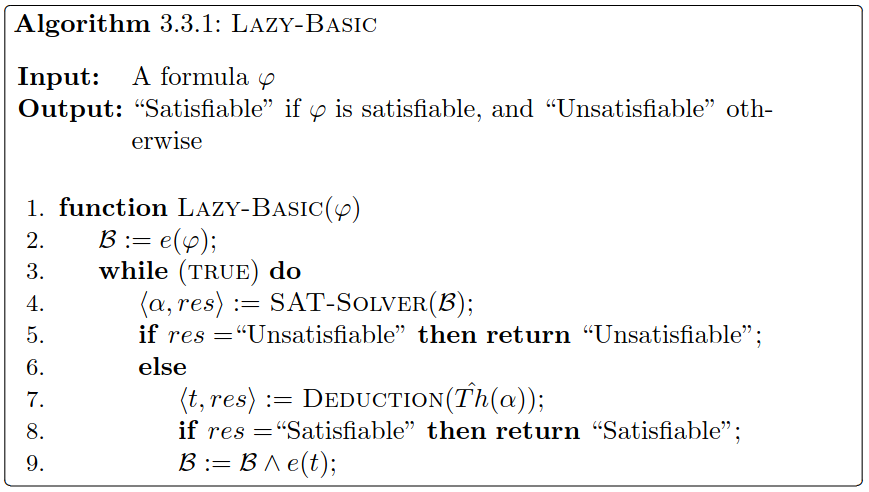
\includegraphics[width=15.5cm]{images/LazyAlgorithm.png}  
\end{center}
\\
\\
2. Сначала вычислим $B = e(\phi)$ \\
4. Отправляем результат вычисления $B$ SAT-решателю.\\
5. Если получили "UNSAT", то возвращаем "UNSAT".\\
7. Иначе вычисляем $Deduction(\hat{Th(\alpha)})$ \\
8. Если Deduction вернул "SAT", то возвращаем "SAT" \\
9. Если Deduction вернул "UNSAT", то добавляем в $B$ блокирующий дизъюнкт, который позволяет больше не учитывать данное решение(это решение нам не подходит и блокирующий дизъюнкт гарантирует, что мы больше его не получим).\\

}
\end{blockquote}

% Вопрос №10	
\Pr[\textcolor{mygreen}{Каринэ, DONE}] Что такое правило единичного дизъюнкта?
			
\solution{10}
\begin{blockquote}
{\color{myblue}

\textcolor{mypurpur}{\textit{Взято из \url{https://www.cs.princeton.edu/~zkincaid/courses/fall18/readings/SATHandbook-CDCL.pdf}, стр. 129 и видео 6 лекции}}\\

\noindent \textbf{\textit{Единичный дизъюнкт}} -- это дизъюнкт, в котором все литералы кроме одного равны 0, а оставшемуся литералу значение не присвоено. \\
\textbf{\textit{Правило единичного дизъюнкта}}  -- если дизъюнкт единичный, то единственному неопределенному литералу нужно присвоить значение 1, чтобы дизъюнкт стал выполнимым.
\\ \\
 \textit{Пример:} \\
 Пусть дано частичное определение
 \[\{x_1 \mapsto 1, x_2 \mapsto 0, x_4 \mapsto 1\}\]
 Тогда \\ 
 \((x_1 \vee x_3\vee\neg{x_4})\) - выполнимый дизъюнкт \\
\((\neg{x_1} \vee x_2)\) - конфликтный дизъюнкт \\
\((\neg{x_1}\vee\neg{x_4}\vee x_3)\) - \textbf{единичный дизъюнкт} \\
\((\neg{x_1}\vee x_3\vee x_5)\) - неразрешенный дизъюнкт


}



\end{blockquote}

% Вопрос №11		
\Pr[\textcolor{mygreen}{Паша, DONE}] Опишите $CDCL$ алгоритм.
			
\solution{11}
\begin{blockquote}
{\color{myblue}
\textbf{\textit{Conflict-driven clause learning}}

\begin{figure}[H]
    \centering
    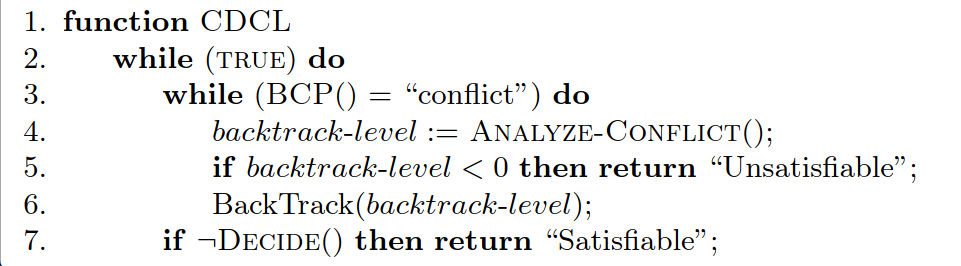
\includegraphics[width=0.7\linewidth]{images/CDCL.png}
    \label{ris:cdcl}
\end{figure}

\textbf{BCP()} - (BackTrackingPropagation) оценивает все переменные из единичных дизъюнктов, если конфликт произошел, то будет произведена попытка отката

\textbf{Decide()} - подбрасывает монетку и делает предположение о какой-то переменной (если всё оценено, то возвращает \textit{True})

\textbf{Analyze-Conflict()} - строит блокирующий дизъюнкт, добавляет его к исходной формуле, и смотрит на какой уровень нужно откатиться

\textbf{BackTrack()} - откатывается на нужный уровень
}
\end{blockquote}

% Вопрос №12		
\Pr[\textcolor{mygreen}{Саит, DONE}] Что такое граф следствий?
			
\solution{12}
\begin{blockquote}
{\color{myblue}
\textcolor{mypurpur}{\textit{На основе "Лекции 6. Оптимизации CDCL". И Decision Procedures, страница $33$.}}\\
\\
\noindent \textbf{\textit{Граф следствий}} -- это ациклический, ориентированный граф $G(V, E)$ с пометками на ребрах, такой, что:
\begin{itemize}
    \item Вершины графа - переменные, определенные частичной оценкой.
    \item Будем обозначать вершины $x_i @ dl$, если на уровне $dl$ мы присвоили переменной $x_i$ значение истина и $\neg{x_i} @ dl$ - если присвоили ложь.
    \item Из вершины $v_i$ идет ребро в вершину $v_j$ , если переменная $v_j$ оценена на основе дизъюнкта $c$ и $v_i$ входит в $c$. Это ребро помечается меткой $c$.
    \item Если есть конфликт, то ему соответствует вершина \textbf{К}. Пусть $c$ - конфликтный дизъюнкт. Тогда к вершине \textbf{К} идут ребра от переменных, входящих в $c$ и они помечаются меткой $c$.
\end{itemize}

Граф следствий служит для того, чтобы проиллюстрировать процесс распространения единиц \textit{(Boolean constraint propagation, BCP())} в $CDCL$ алгоритме.

На рисунке~\ref{ris:graph_cdcl} представлен пример графа следствий:
\begin{figure}[H]
    \centering
    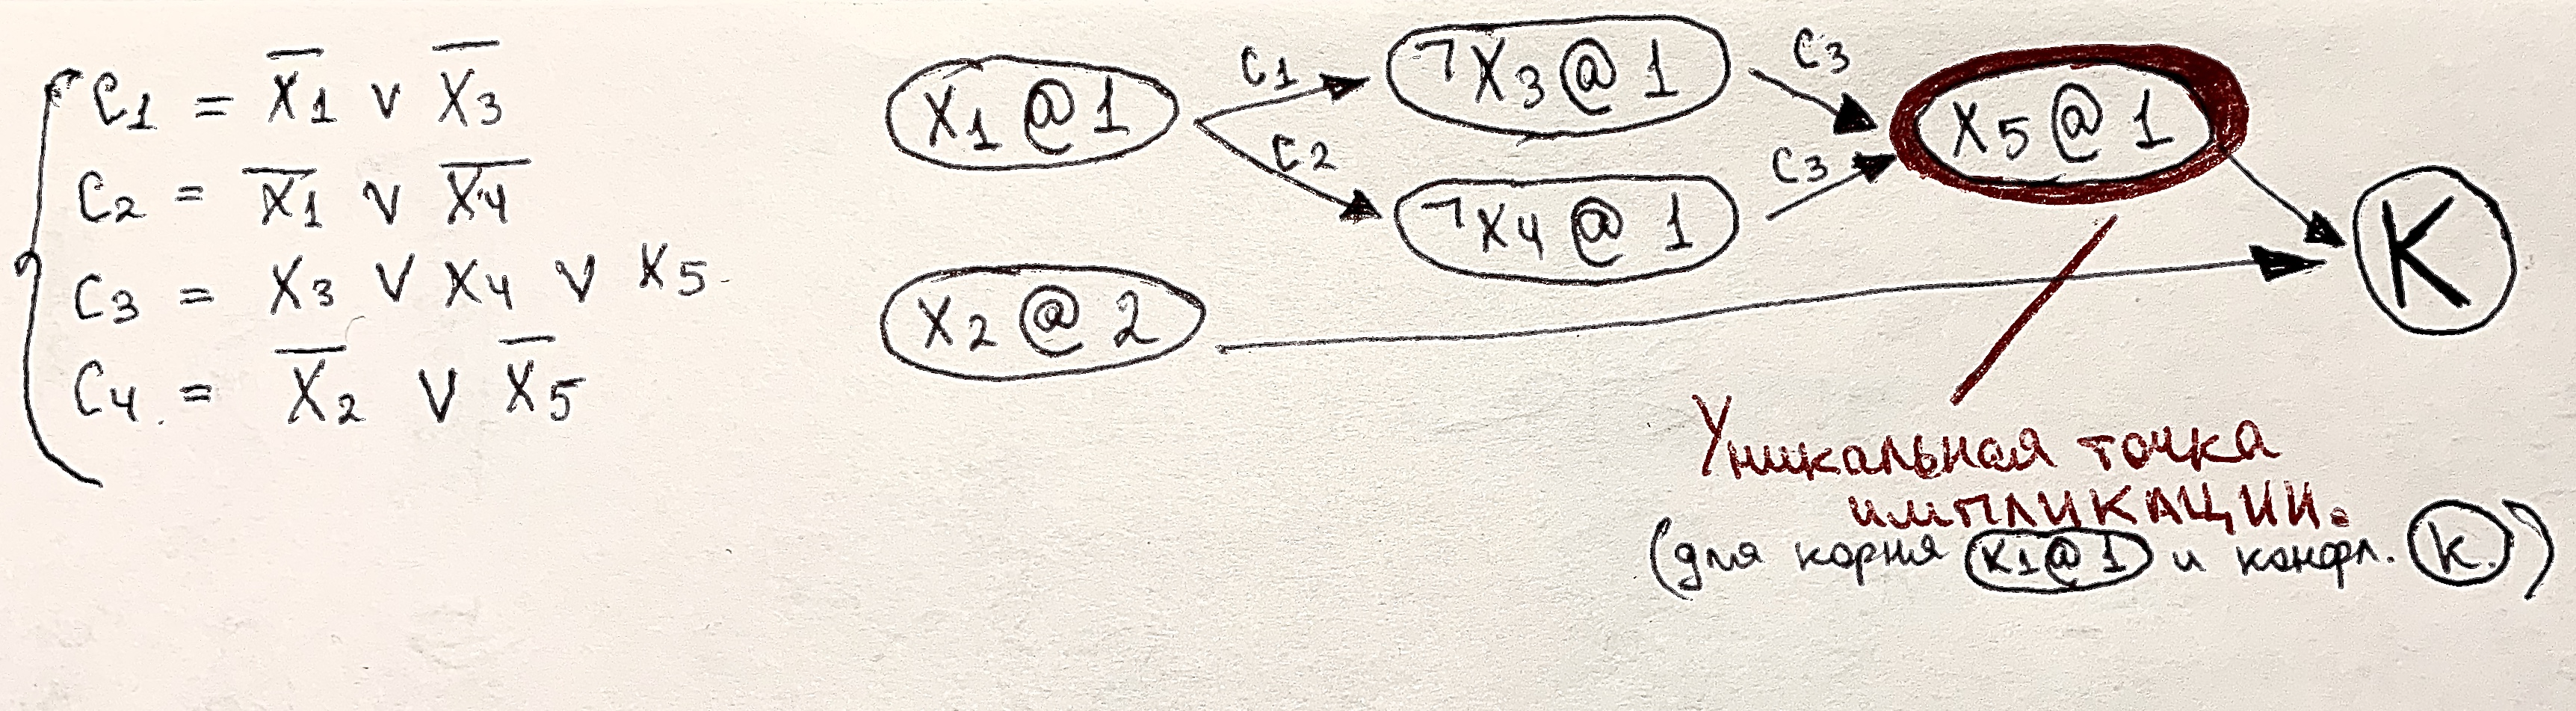
\includegraphics[width=16.5cm]{images/graph_cdcl.JPG}
    \caption{Граф следствий. Красным цветом помечена уникальная точка импликации для корня $x_1 @ 1$ и указанной вершины \textit{"конфликт"}.}
    \label{ris:graph_cdcl}
\end{figure}
}
\end{blockquote}

% Вопрос №13			
\Pr[\textcolor{mygreen}{Алтана, DONE}] Что такое уникальная точка импликаций?
			
\solution{13}
\begin{blockquote}
{\color{myblue}
\textcolor{mypurpur}{\textit{На основе "Лекции 6. Оптимизации CDCL"}}\\
\\
\noindent \textbf{\textit{Уникальная точка импликации}} -- любая вершина графа  следствий (импликаций), которая не является вершиной \textit{«конфликт»} и которая находится на каждом пути, ведущему от конкретной корневой вершины к конкретной вершине \textit{«конфликт»}.\\
\\
На рисунке~\ref{ris:graph_cdcl} представлен пример графа следствий и уникальной точки импликации.
}
\end{blockquote}

% Вопрос №14		
\Pr[\textcolor{mygreen}{Каринэ, DONE}] Опишите DPLL(T) алгоритм.
			
\solution{14}
\begin{blockquote}
{
\color{myblue}
\textcolor{mypurpur}{\textit{Лекция 7, Decision Procedures, страница $67$.}} \\
\noindent 
\\
\textbf{Основная идея неформально:} \\ \\
\textit{Предположим, получили частичную оценку формулы. Теперь нужно проверить, непротиворечива ли она. Основная идея состоит в том, что  в Lazy-CDCL  Deduction вынесена из if и производится всегда, когда отрабатывает внутренний while и получается какая-то оценка. Если получилась невыполнимая формула, то делается back tracking и формула добавляется в блокирующий класс. (Получился алгоритм DPLL(T)). Это может увеличить время работы алгоритма. Для ускорения можно применять эвристики - вызывать Deduction не всегда, а если оценено определенное количество переменных. Этот солвер может искать минимально противоречивое ядро - количество атомов, которые нужно \glqq запретить\grqq} \\ \\
\textbf{Более формальное описание:} \\
Ленивый CDCL: 
\begin{center}
  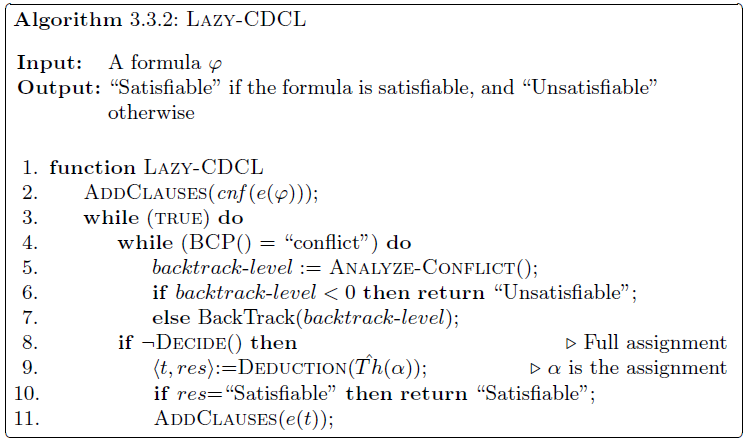
\includegraphics[width=13cm]{images/Lazy_cdcl.png}  
\end{center}


Ленивый CDCL алгоритм может быть улучшен вызовом Deduction
перед булевым кодированием. Такой ранний вызов служит двум целям:
\begin{itemize}
    \item Противоречивые частичные оценки исключаются на ранней стадии
    \item Значения литералов, которые еще не были оценены могут быть переданы обратно в SAT солвер, т.е. информация сохранена и может быть использована дальше.
\end{itemize}

Таким образом, мы приходим к алгоритму \textbf{DPLL(\textit{T})} \\ 
\par
Дано:
\begin{itemize}
    \item $at(\phi)$ - множество атомов в формуле $\phi$
    \item $at_i(\phi)$ - определенный атом из этого множества.
    \item Атом $a$ сопоставляем с булевой переменной $e(a)$ (такая процедура называется булевским кодированием).
    \item $e(t)$ - булева формула, полученная булевым кодированием каждого атома формулы $t$.
    \item $\alpha$ - некоторая(возможно, частичная) оценка формулы $e(\phi)$
    \item 
    \begin{equation*}
        Th(at_i, \alpha) =
        \begin{cases}
          at_i & \alpha(at_i) = TRUE \\
          \neg at_i & \alpha(at_i) = FALSE
        \end{cases}
    \end{equation*}
    \item $Th(\alpha) = {Th(at_i, \alpha | e(at_i), \alpha)}$
    \item $\hat{Th(\alpha)}$ - конъюнкция всех элементов из $Th(\alpha)$
\end{itemize}
\begin{center}
  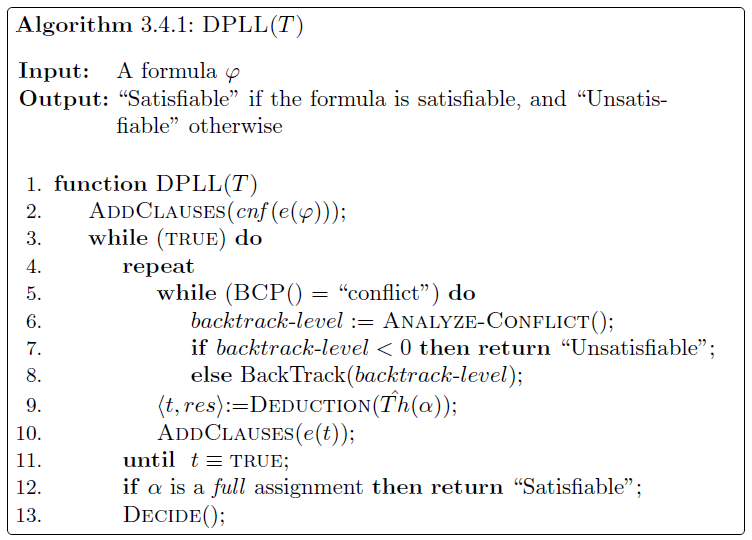
\includegraphics[width=13cm]{images/DPLL.png}  
\end{center}

Здесь Deduction вызывается в 9 строке, когда с помощью BCP уже не будет сделано никаких оценок. Далее находятся \textit{T}-оцененные литералы и передаются в CDCL часть солвера в форме ограничений. Поэтому, в дополнение к следствиям в булевом домене, здесь также возникают следствия, связанные с теорией \(T\). Соответственно, данная техника называется \textbf{распространение теорий.} \par 

Требования к добавляемым дизъюнктам: они должны следовать из \(\phi\) и ограничены конечным множеством атомов. Желательно, чтобы в случае неразрешимости \(\hat{Th(\alpha)}\), \(e(t)\) блокировала \(\alpha\); это не является обязательным, потому что блокировка или не блокировка \(\alpha\) не влияет на корректность - Deduction завершается только когда \(\alpha\) - полная оценка. В случае, когда  \(\hat{Th(\alpha)}\) выполнима, требуется чтобы \(t\) удовлетворяло одному из двух следующих условий для того, чтобы гарантировать остановку работы алгоритма:
\begin{itemize}
    \item Добавление \(e(t)\) в \(\bm{\mathcal{B}}\) и вызов BCP ведет к оценке некоторого литерала.
    \item Когда Deduction не может найти дизъюнкт, удовлетворяющий первому условию, \(t\) и \(e(t)\) эквивалентны TRUE.
\end{itemize}

Второй случай возникает, например, когда булевы переменные уже оценены, и, следовательно, формула является выполнимой. В таком случае выполняется условие в строке 11 и процедура продолжается с 13 строки, где снова вызывается Decide. Поскольку все переменные уже оценены, процедура возвращает \glqq Satisfiable\grqq. \\


\par 
\textit{Пример:} \\ \par
Рассмотрим случай двух булевых формул \(e(x_1\geq 10)\) и \(e(x_1<0)\). После того, как первая формула была установлена в TRUE, процедура Deduction делает вывод, что формула
\[t :=\neg{(x_1\geq 10)}\vee\neg{(x_1<0)}\]
является T-допустимой. Тогда соответствующая \(t\) булева формула \[e(t):=(\neg{e(x_1\geq 10)}\vee\neg{e(x_1<0)})\]
добавляется в \(\bm{\mathcal{B}}\), что приводит к незамедлительному следствию \(\neg{e(x_1<0)}\) и, возможно, дальнейшим следствиям.
}

\end{blockquote}

% Вопрос №15		
\Pr[Паша] Опишите разрешающую процедуру для теории равенства и неинтерпретируемых функций.
			
\solution{15}
\begin{blockquote}
{\color{myblue}
\noindent \textbf{Алгоритм}\\
\textbf{Вход: } $\phi^{UF}$ - конъюнкция предикатов равенства (я так понял неравенства тоже) над переменными и неинтерпретируемыми
функциями.\\
$$
\phi^{UF}:=x_1=x_2 \wedge x_2=x_3 \wedge x_4 = x_5 \wedge x_5 \neq x_1 \wedge F(x_1) \neq F(x_3)
$$
% 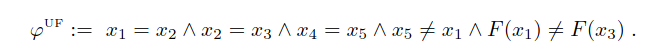
\includegraphics[width=13cm]{images/congruence_0.png}\\  
\textbf{Выход: } $SAT/UNSAT$.
\begin{enumerate}
    \item Возьмем два терма $t_1, t_2$ (это могут быть как переменные, так и неинтерпретируемые
    функции) и отнесем их в один класс эквивалентности, если в $\phi^{UF}$ встречается предикат
    $t_1 = t_2$. Оставшиеся термы будут образовывать одноэлементные классы эквивалентности. (В данном пункте подразумевается, что мы будем как бы идти по предикатам и для каждой парочки создавать свой класс).\\
    $$
    \{x_1, x_2\},\{x_2, x_3\}, \{x_4, x_5\},\{F(x_1)\},\{F(x_3)\}
    $$
    % 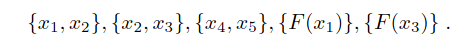
\includegraphics[width=13cm]{images/congruence_1.png}\\ 
    \item Пройдемся по получившимся классам. Если у каких-то классов есть общий терм, объединяем
    их в один общий класс. Повторяем до тех пор, пока мы можем это делать.\\
    $$
    \{x_1, x_2, x_3\},\{x_4, x_5\},\{F(x_1)\},\{F(x_3)\}
    $$
    % 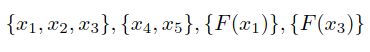
\includegraphics[width=13cm]{images/congruence_2.png}\\ 
    \item Пройдемся по получившимся классам. Если термы $t_i, t_j$ лежат в одном классе, а также 
    в $\phi^{UF}$ встречаются термы $F(t_i), F(t_j)$ (где $F$ - некоторая неинтерпретируемая функция), то объединяем классы, представителями которых являются $F(t_i)$ и $F(t_j)$.
    Повторяем до тех пор, пока можем.\\
    $$
    \{x_1, x_2, x_3\},\{x_4, x_5\},\{F(x_1), F(x_3)\}
    $$
    % 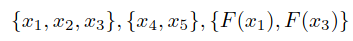
\includegraphics[width=13cm]{images/congruence_3.png}\\ 
    \item Если в $\phi^{UF}$ присутствует предикат $t_i \neq t_j$, такой, что $t_i, t_j$ принадлежат одному классу эквивалентности, то возвращаем $UNSAT$. Иначе - $SAT$.
    
\end{enumerate}

}
\end{blockquote}

% Вопрос №16		
\Pr[\textcolor{mygreen}{Саит, DONE}] Какой метод лежит в основе разрешающей процедуры теории линейной арифметики?

\solution{16}
\begin{blockquote}
{\color{myblue}
\noindent \textcolor{mypurpur}{\textit{На основе лекции $8$.}}\\			
\\
\noindent Симплекс метод.
}
\end{blockquote}

% Вопрос №17			
\Pr[Алтана] Что такое комбинация теорий?
			
\solution{17}
\begin{blockquote}
{\color{myblue}
\noindent 

Теория $T$ -- это множество "предложений"(формулы 1-го порядка над сигнатурой $\Sigma$, где все переменные связаны с квантором)

Пусть $T_1$, $T_2$ - теории над сигнатурами $\Sigma_1$, $\Sigma_2$ соответственно. Тогда \textbf{комбинацией теорий} $T_1 \oplus T_2$ назовем теорию над сигнатурой $\Sigma_1\cup\Sigma_2$ над множеством аксиом $T_1\cup T_2$
}
\end{blockquote}

% Вопрос №18		
\Pr[\textcolor{mygreen}{Каринэ, DONE}] Что такое выпуклые теории?
			
\solution{18}
\begin{blockquote}
{\color{myblue}
\noindent  \textcolor{mypurpur}{\textit{ Определение из Decision procedures, стр. 230 и лекции 10}}\\ \\
\(\Sigma\) - теория \(T\) является \textbf{\textit{выпуклой}}, если для любой \(\Sigma\)-формулы \(\phi\) \\
\((\phi \Rightarrow \bigvee\limits_{i=1}^{n} x_i=y_i)\) - \(T\) - тавтология для некоторого конечного \(n>1\Rightarrow\) \\
\((\phi \Rightarrow x_i=y_i)\) - \(T\) - тавтология для некоторого \(i \in \{1,\dots,n\}\) \\
где \(x_i,y_i, i\in\{1,\dots,n\}\) - некоторые переменные. \\ \\
Другими словами, в выпуклой теории \(T\), если формула подразумевает дизъюнкцию равенств, то она 
подразумевает также хотя бы одно из этих равенств по отдельности.

}
\end{blockquote}

% Вопрос №19		
\Pr[Паша] Что такое ограничение Нельсона-Оппена?
			
\solution{19}
\begin{blockquote}
{\color{myblue}
\textbf{\textit{Ограничения Нельсона-Оппена:}}
\begin{enumerate}
    \item $T_1, ..., T_n$ - бескванторные теории с равенством
    \item Для каждой теории есть разрешающая процедура
    \item Пересечение каждой пары сигнатур - пустое множество
    \item Теории интерпретируются над бесконечным доменом (теории вида битовых векторов не подходят)
    \item[P.S.] Интерпретация тоже задана \textit{(хз органичение или нет)}
\end{enumerate}
}
\end{blockquote}

% Вопрос №20		
\Pr[\textcolor{mygreen}{Саит, DONE}] Что такое вычислительное дерево программы?
			
\solution{20}
\begin{blockquote}
{\color{myblue}
\textcolor{mypurpur}{\textit{Есть в лекции $11$, но там нет видео.}}\\
\\
\noindent \textbf{\textit{Вычислительное дерево программы}} -- способ представления программы в виде бинарного дерева, при котором:
\begin{itemize}
    \item Каждая вершина - выполнение условного оператора.
    \item Каждое ребро -- выполнение последовательности команд, которые не являются условным оператором.
\end{itemize}
Таким образом, каждый путь от корня делит множество входных данных на классы эквивалентности.
}
\end{blockquote}

% Вопрос №21			
\Pr[\textcolor{mygreen}{Алтана, DONE}] Что такое путь исполнения программы?
			
\solution{21}
\begin{blockquote}
{\color{myblue}
\textcolor{mypurpur}{\textit{Есть в лекции $11$, но там нет видео.}}\\
\\
\noindent \textbf{\textit{Вычислительное дерево программы}} -- способ представления программы в виде бинарного дерева, при котором:
\begin{itemize}
    \item Каждая вершина - выполнение условного оператора.
    \item Каждое ребро -- выполнение последовательности команд, которые не являются условным оператором.
\end{itemize}

\noindent \textbf{\textit{Путь исполнения программы}} -- это путь от корня до какого-либо листа в  вычислительном дереве программы.
}
\end{blockquote}

% Вопрос №22		
\Pr[\textcolor{mygreen}{Паша, DONE}] Дана программа, выпишите все пути исполнения программы.
			
\solution{22}
\begin{blockquote}
{\color{myblue}

\begin{center}
  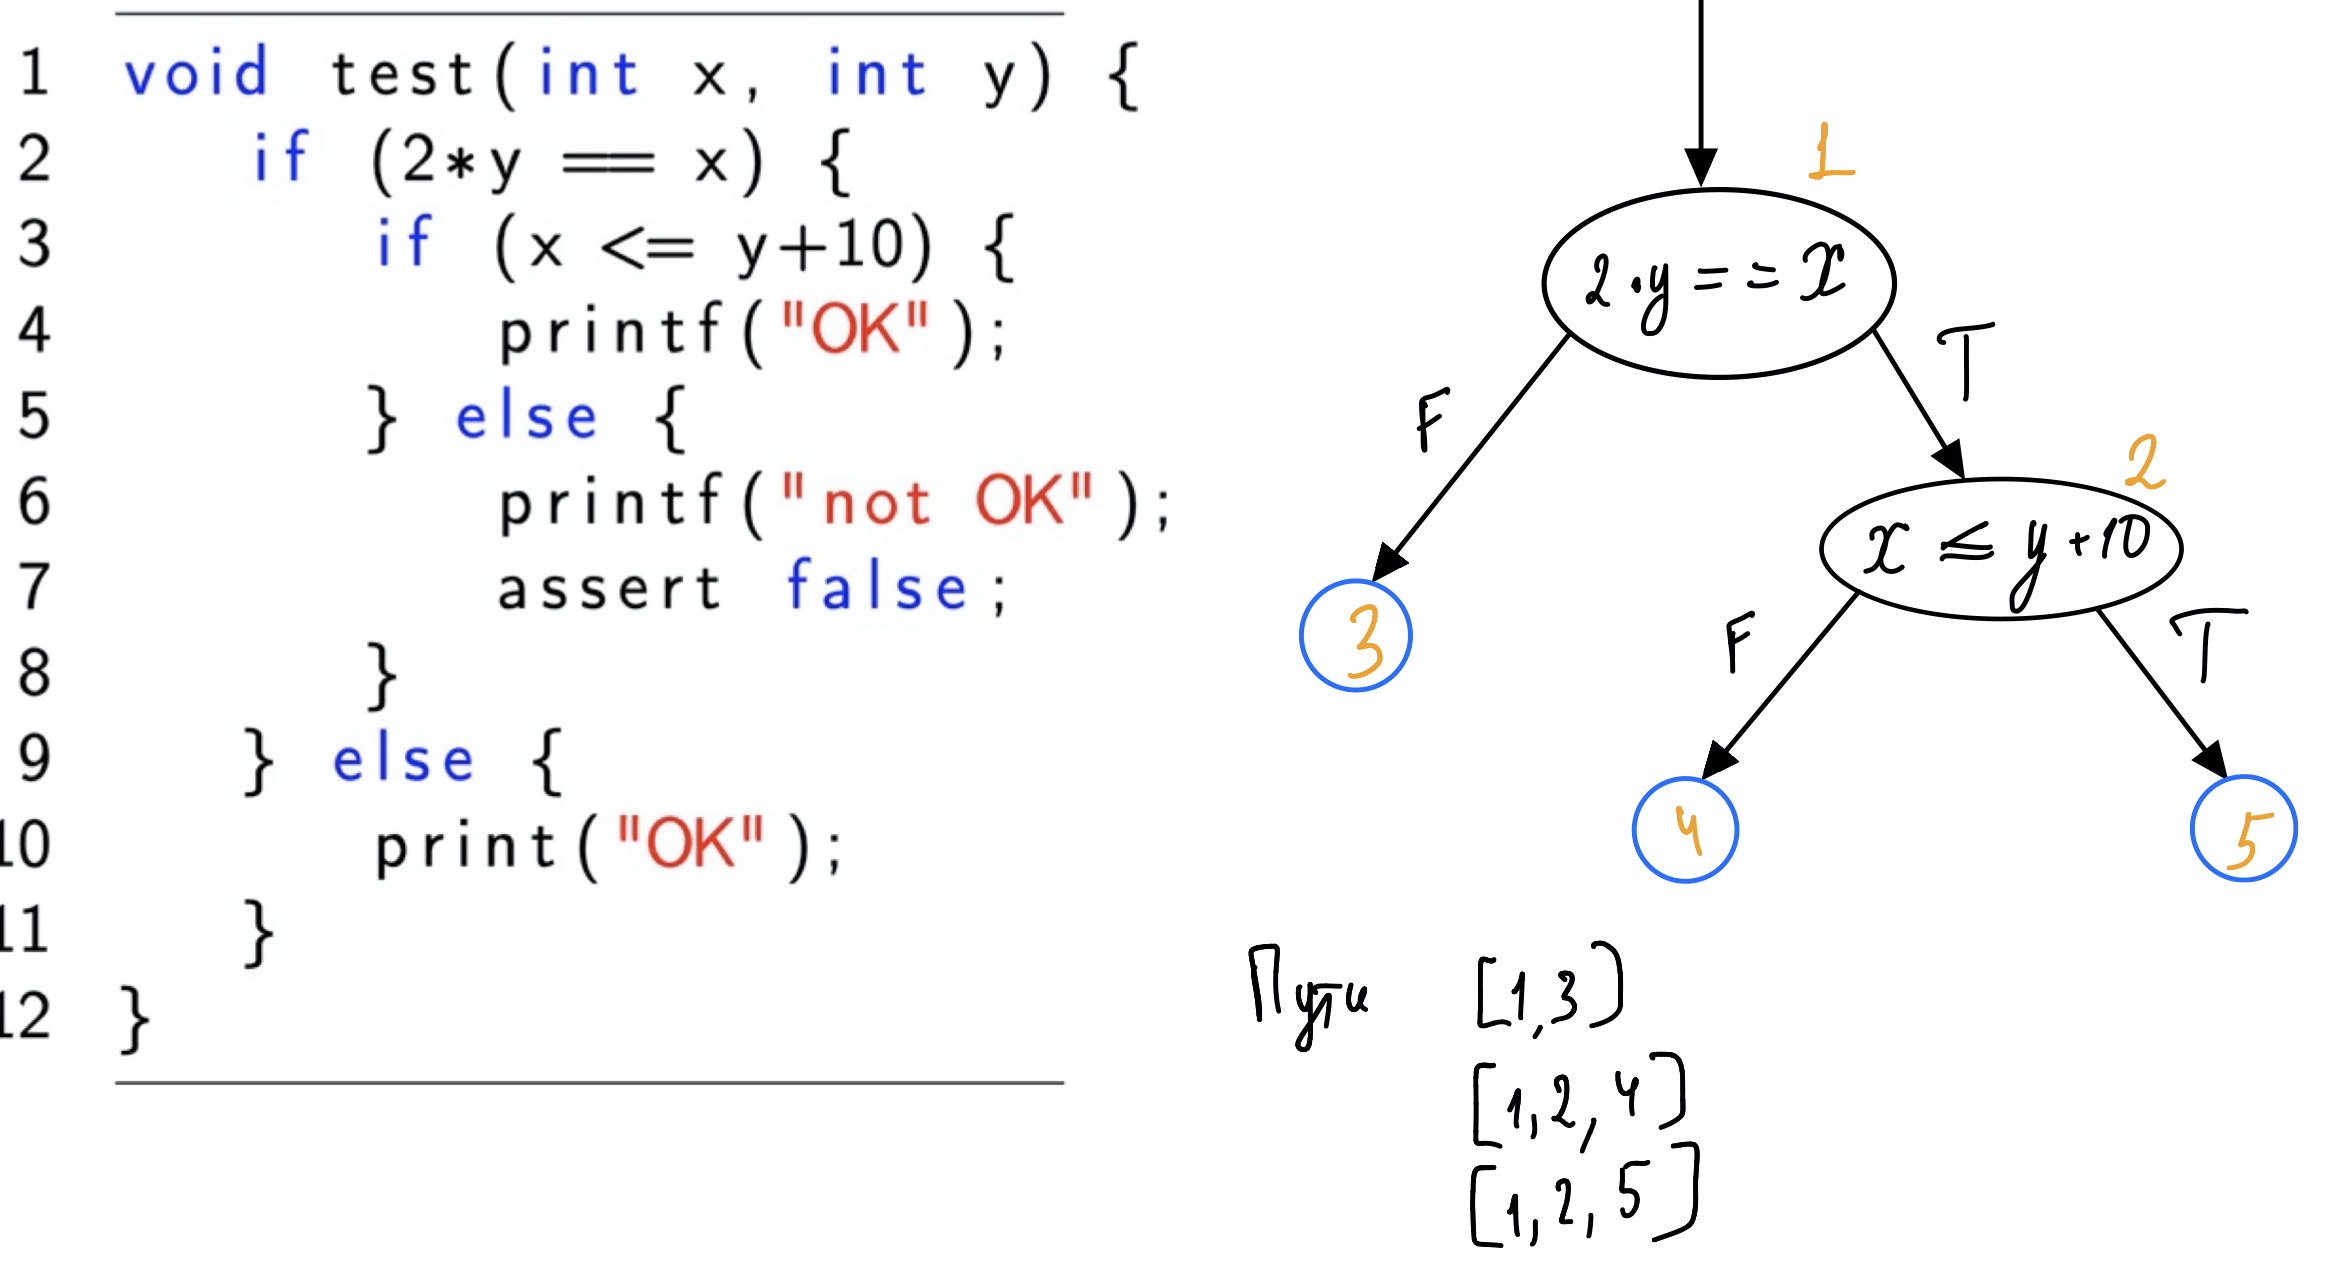
\includegraphics[width=0.8\linewidth]{images/prog_graph.jpeg}  
\end{center}

}
\end{blockquote}

% Вопрос №23		
\Pr[\textcolor{mygreen}{Саит, DONE}] Дана программа, выпишите её path constaint.

\solution{23}
\begin{blockquote}
{\color{myblue}
\textcolor{mypurpur}{\textit{На основе лекции $12$.}}\\
\\
\noindent \textbf{\textcolor{orange}{Пример 1:}}\\
\noindent Дана следующая программа. Суть в том, что в данные разбиты на блоки, в начале каждого блока ссылка на начало следующего блока.
\begin{lstlisting}
void ReadBlocks (int data[], int cookie) {
    int i = 0;
    while (true) {
        int next;
        next = data[i];
        if (! (i < next && next < N)) return;
        i = i + 1;
        for (; i < next; i = i + 1) {
            if (data[i] == cookie) { // skip data
                i = i + 1;
            }
            else { // process data
                Process(data [i]);
            }
        }
    }
}
\end{lstlisting}
Рассмотрим ее следующую \textbf{трассу} (видимо в таком задании будет дана трасса):
\begin{lstlisting}
i = 0;                      // 2, assignment
next = data[i];             // 5, assignment
i < next && next < N        // 6, branch
i = i + 1;                  // 7, assignment
i < next                    // 8, branch
data[i] != cookie           // 9, branch
Process(data[i]);           // 13, function call
i = i + 1;                  // 8, assignment
!(i < next)                 // 8, branch
next = data[i];             // 5, assignment
!(i < next && next < N)     // 6, branch
\end{lstlisting}
Далее по этой трассе можно построить \textbf{\textit{SSA (Static single assignment)}} -- для этого каждый раз, когда происходит новое присваивание, мы вводим новую перемнную. Все это нужно для того, чтобы представить трассу в виде формулы, которую можно будет отдать солверу и получить от него набор переменных, которые удовлетворяют данной трассе.\\
\textbf{\textit{SSA}} для приведенной выше трассы:
\begin{lstlisting}
i_1 = 0;                        // 2, assignment
next_1 = data_0[i_1];           // 5, assignment
i_1 < next_1 && next_1 < N_0    // 6, branch
i_2 = i_1 + 1;                  // 7, assignment
i_2 < next_1                    // 8, branch
data_0[i_2] != cookie_0         // 9, branch
Process(data_0[i_2]);           // 13, function call
i_3 = i_2 + 1;                  // 8, assignment
!(i_3 < next_1)                 // 8, branch
next_2 = data_0[i_3];           // 5, assignment
!(i_3 < next_2 && next_2 < N_0) // 6, branch
\end{lstlisting}
А уже по полученному SSA мы можем легко получить \textbf{\textit{Path constraint}}:\\
\\
\begin{tabular}{l l}
$i_1 = 0 & \wedge$\\
$next_1 = data_0[i_1] & \wedge$\\
$(i_1 < next_1 \wedge next_1 < N_0) & \wedge$\\
$i_2 = i_1 + 1 & \wedge$\\
$i_2 < next_1  & \wedge$\\
$data_0[i_2] \neq cookie_0 & \wedge$\\
$i_3 = i_2 + 1 & \wedge$\\
$\neg(i_3 < next_1) & \wedge$\\
$next_2 = data_0[i_3] & \wedge$\\
$\neg(i_3 < next_2 \wedge next_2 < N_0)$\\
\end{tabular}\\
\\
\\
\noindent \textbf{\textcolor{orange}{Пример 2:}}\\
Можно анализировать программы на то, что все assert-ы в них никогда не срабатывают или находить примеры, на которых они срабатывают. Для этого достаточно добавить отрицание условия в соответствующем assert в path constraint и отдать все это солверу. Если получим SAT и набор переменных, то assert сработал, а если получим UNSAT, то все ок -- assert никогда не срабатывает.\\
\\
Рассмотрим следующую, другую трассу вышеприведенной программы:
\begin{lstlisting}
i = 0;                  // 2, assignment
next = data[i];         // 5, assignment
i < next && next < N    // 6, branch
i = i + 1;              // 7, assignment
i < next                // 8, branch
data[i] = cookie        // 9, branch
i = i + 1;              // 10, assignment
i = i + 1;              // 8, assignment
!(i < next)             // 8, branch
0 <= i && i < N         // 5, assertion
\end{lstlisting}
Видим, что в последней строчке мы хотим видеть assert для $0 <= i \wedge i < N$, прежде чем обращаться к $next = data[i]$, рискуя выйти за границы массива $data$.\\
Окей, просто добавим отрицание этого assert к path constraint (шаг с построением SSA выполняем в уме):\\
\begin{tabular}{l l}
$i_1 = 0 & \wedge$\\
$next_1 = data_0[i_1] & \wedge$\\
$(i_1 < next_1 \wedge next_1 < N_0) & \wedge$\\
$i_2 = i_1 + 1 & \wedge$\\
$i_2 < next_1  & \wedge$\\
$data_0[i_2] = cookie_0 & \wedge$\\
$i_3 = i_2 + 1 & \wedge$\\
$i_4 = i_3 + 1 & \wedge$\\
$\neg(i_4 < next_1) & \wedge$\\
$\neg(0 \leq i_4 \wedge i_4 < N_0)$\\
\end{tabular}\\
\\
\\
\noindent \textbf{\textcolor{orange}{Пример 3:}}\\
Что делать, если у нас цикл ограниченной длины \textit{(Bounded Program Analysis)}?\\
В таком случае мы можем развернуть цикл в несколько вложенных \textit{if}-ов. После этого для того, чтобы переписать нашу программу, чтобы получить логические формулы -- мы будем условия циклов записывать в качестве некоторых переменных, а также будем высчитывать значения необходимые для симуляции поведения того, что было бы если бы мы пошли бы по ветке \textit{True}, а что, если бы по \textit{False}. И далее просто пишем тернарники на переменные согласно \textit{if}-ам:
\begin{figure}[H]
    \centering
    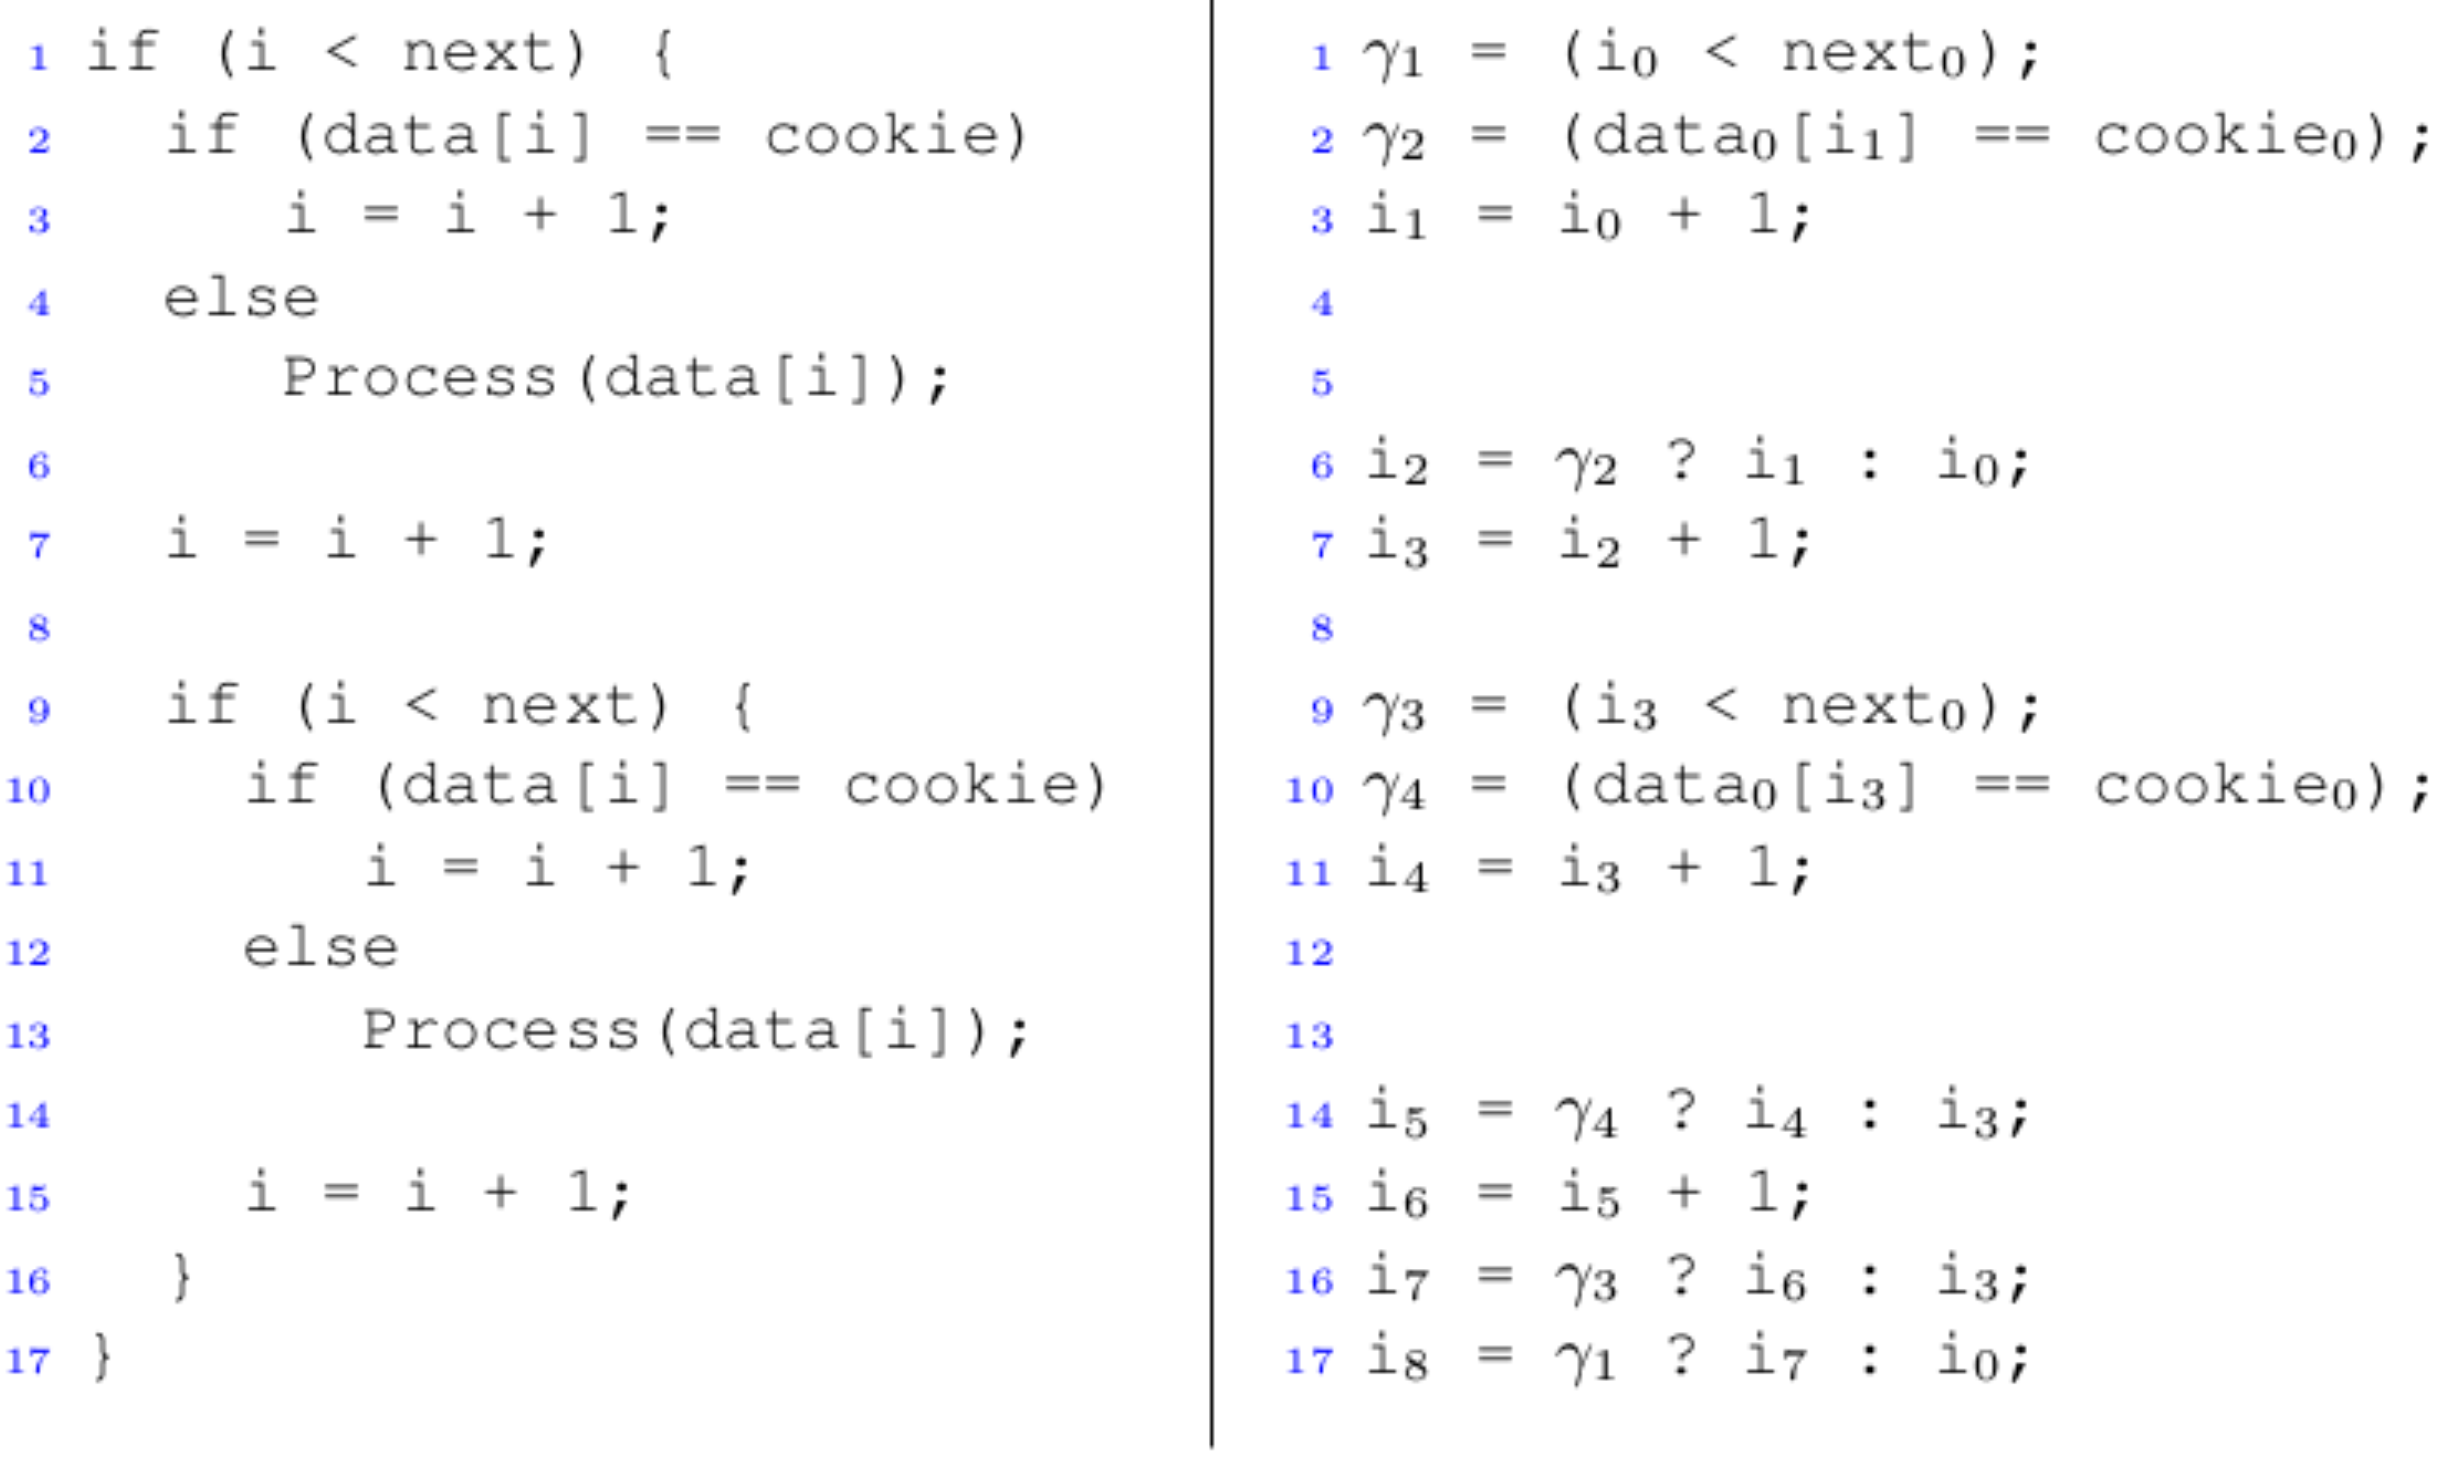
\includegraphics[width=16.0cm]{images/path_constraint01.png}
    \caption{Path constraint для цикла, развернутого в \textit{if}-ы.}
    \label{ris:path_constraint01}
\end{figure}
\noindent \textbf{\textcolor{orange}{Пример 4:}}\\
А что делать, если цикл неограниченной длины, т.е. мы не знаем через сколько именно витков они закончатся \textit{(Unbounded Program Analysis)}?\\
В таком случае мы можем потерять точность в программе, но при этом заменить цикл на \textit{if}:
\begin{figure}[H]
    \centering
    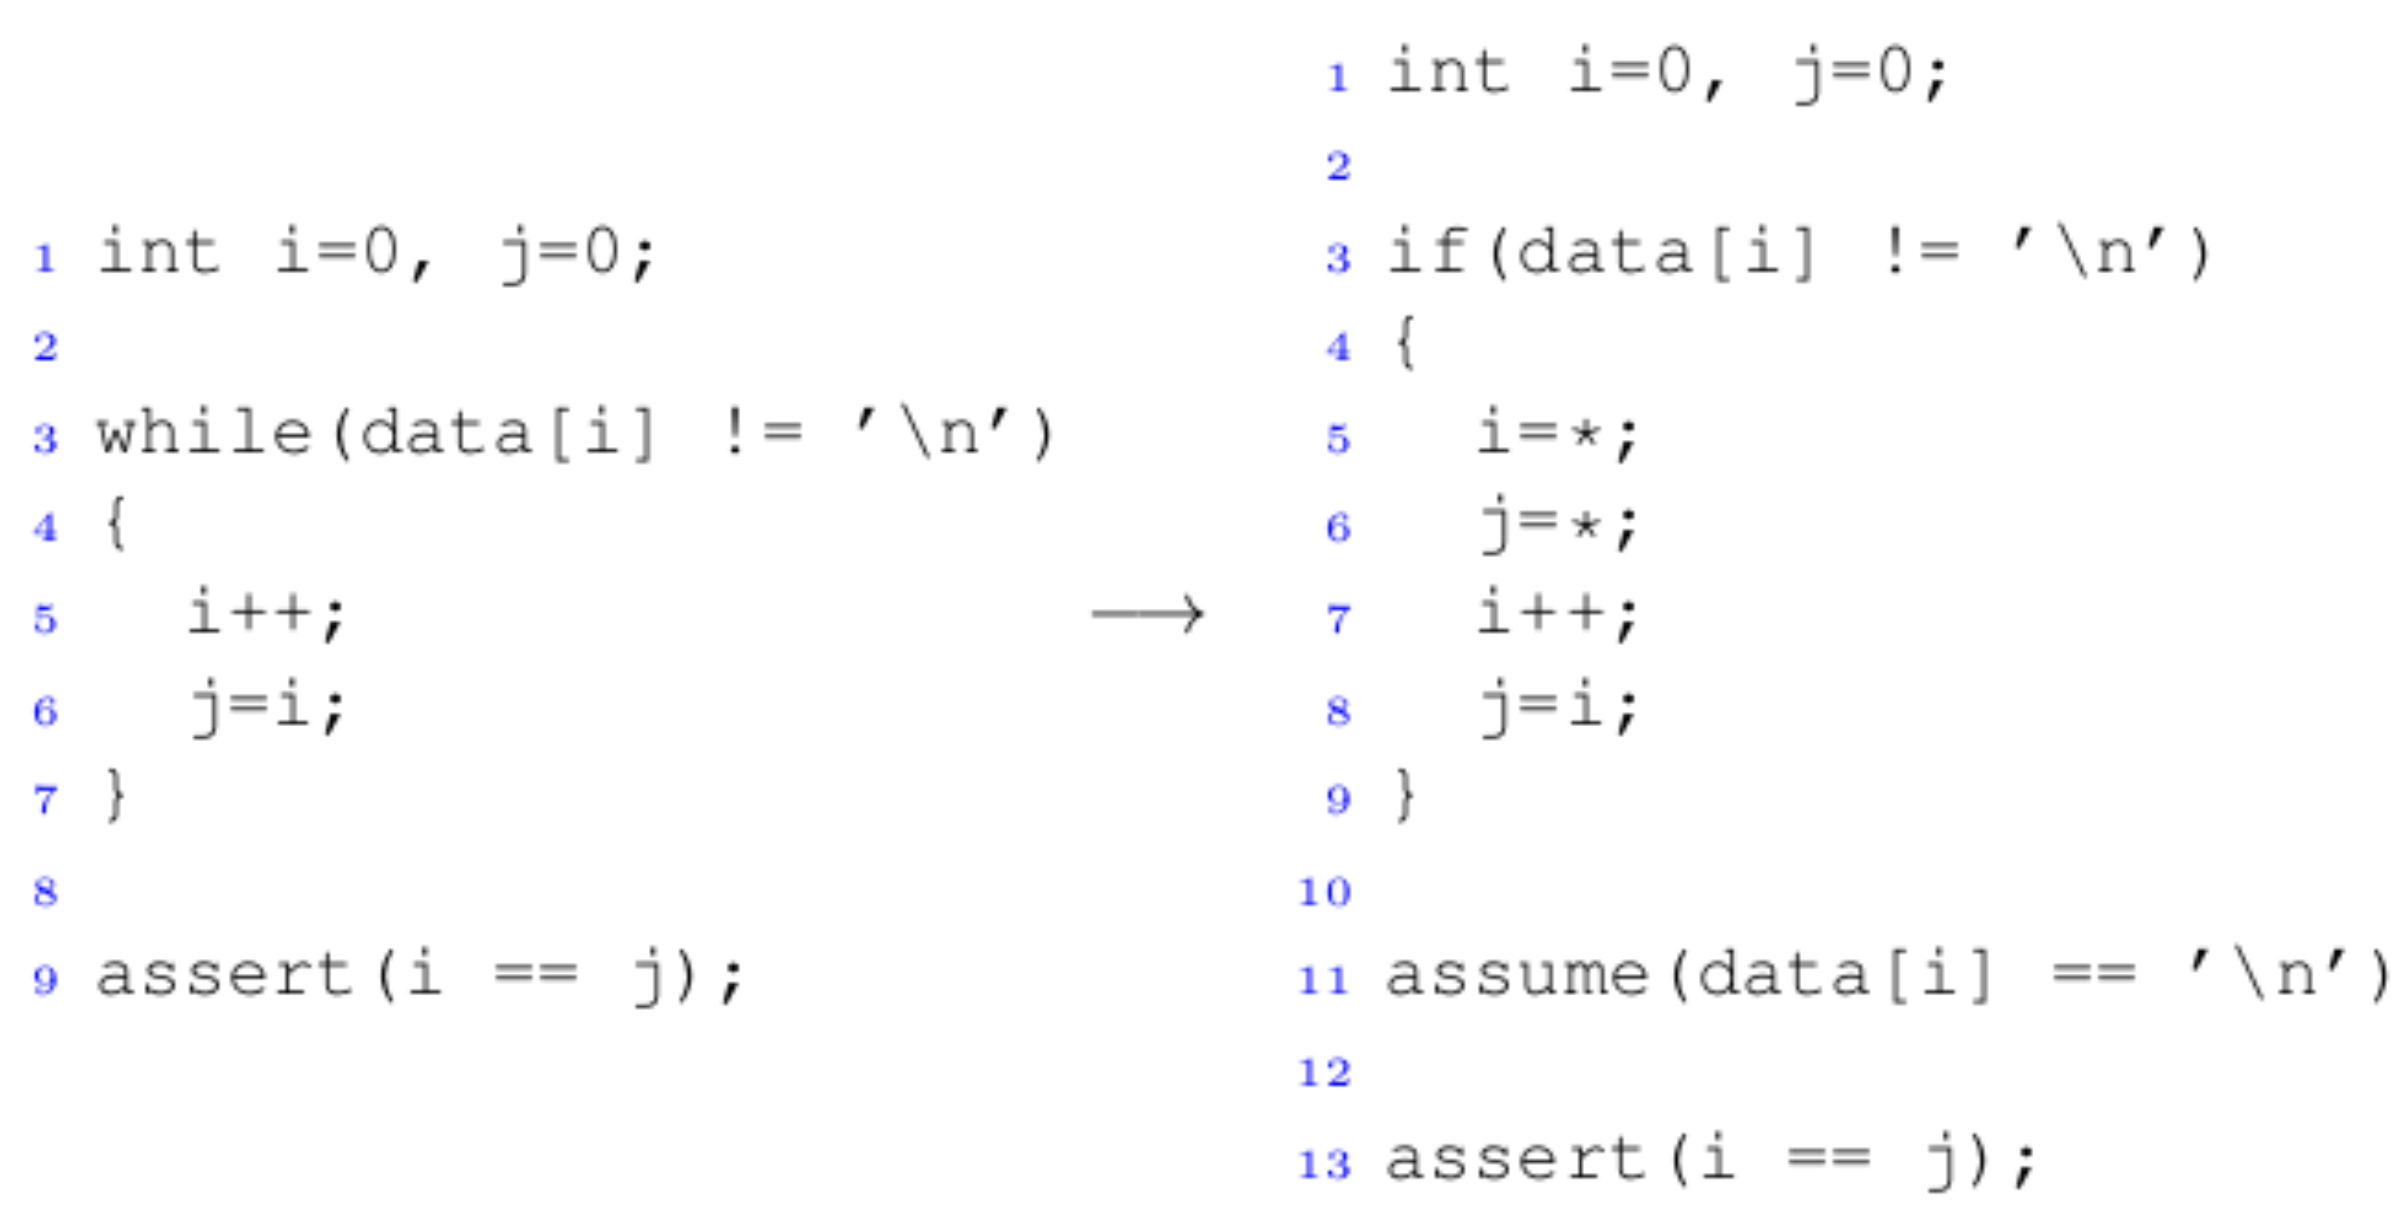
\includegraphics[width=16.0cm]{images/path_constraint02.png}
    \caption{Замена неограниченного цикла.}
    \label{ris:path_constraint02}
\end{figure}
То есть мы сказали, что в \textit{if}-e, в его начале, $i$, $j$ могут быть вообще любыми -- естественно это не совсем так, у них есть свои ограничения, но мы их не учитываем. Наша же цель проверить \textit{assert(i = j)}. В данном случае он будет выполняться всегда и солвер вернут $UNSAT$ на следующий path constraint:\\
\\
\begin{tabular}{l l}
$i_1 = 0 & \wedge$\\
$j_1 = 0 & \wedge$\\
$\gamma_1 = (data_0[i_1] \neq \ '\backslash n') & \wedge$\\
$i_3 = i_2 + 1 & \wedge$\\
$j_3 = i_3 & \wedge$\\
$i_4 = \gamma_1 \ ? \  i_3 : i_1 & \wedge$\\
$j_4 = \gamma_1 \ ? \  j_3 : j_1 & \wedge$\\
$data_0[i_4] = \ '\backslash n' & \wedge$\\
$i_4 \neq j_4$\\
\end{tabular}\\
\\
Заметьте, что $i_2$ и $j_2$ -- действительно любые. При таком подходе мы получаем такое поведение -- если солвер вернет $UNSAT$, то действительно assert никогда не выполнится, но при этом солвер может вернуть $SAT$ и набор переменных, которые не достигаются, но стали возможными из-за того, что мы сделали программу более неточной.
}
\end{blockquote}
			
\end{document}
  